In this chapter expected behavior of product and its resulting requirements will be described. 
First there will be introduced simple life cycle of the product.
Although project title was accepted as a domain and not a final product, following requirements could be applied also on project that is not scaled down.

\section{Description}
To clarify and properly explain life cycle of one run of server side application, its usage and possible requirements, structure of UML's activity diagram \cite{Dumas:2001:UAD:647245.719456} was adopted. 
Therefore we show in figure \ref{img:activity_diagram} interaction between manager and one client user.
Notice that there are some actions of both manager and client user which do require direct manipulation with mobile phone or other actors such as "Notice users to raise their mobiles", "Raise mobile", "Put down mobile" and more.

\begin{figure}[h!]
    \begin{center}
    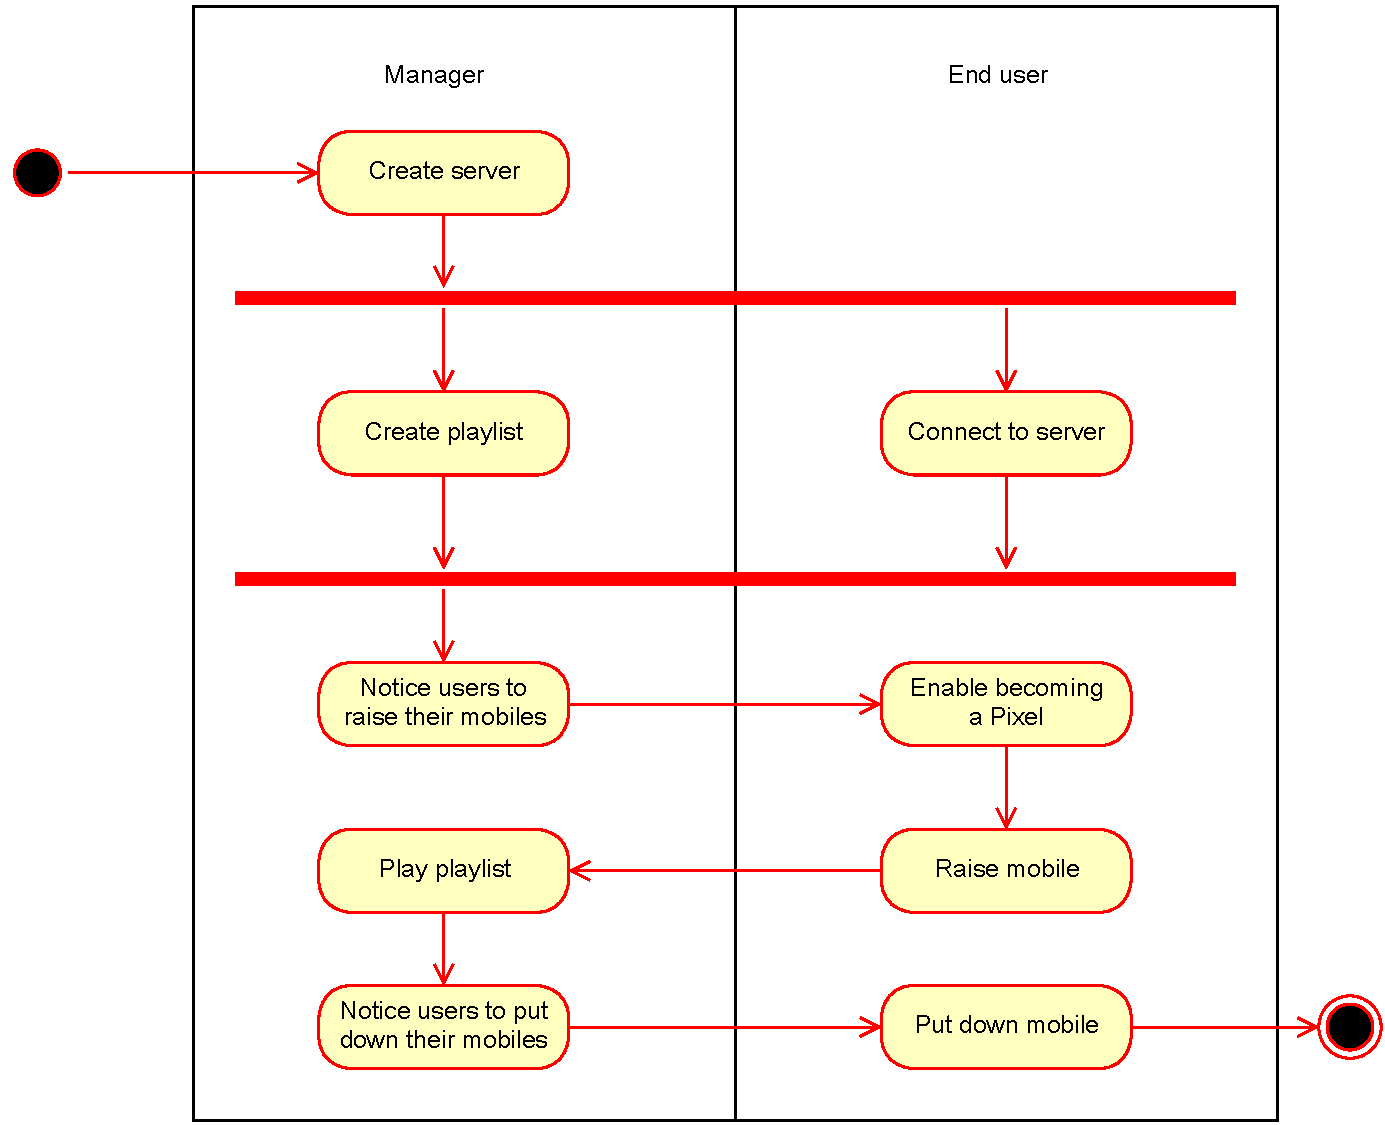
\includegraphics[scale=0.4]{images/activity_diagram.pdf}
    \label{img:activity_diagram}
    \caption{Activity diagram depicting basic scenario of using product with all actors.}
    \end{center}
\end{figure}

\section{Requirements}
Requirements can be divided into two categories \cite[p.~19]{ntnu_req}: functional and non-functional. 
Functional ones describe a function which a system or system component must be able to perform \cite[p.~35]{ieee610.12:1990}.
On the other hand non-functional requirements cover what product is, they are any other requirements than functional  \cite[p.~20]{ntnu_req}.


\subsection{Functional}
In the figure bellow use case diagram \ref{img:usecase} of the whole system  is shown.
According to use case diagram \ref{img:usecase}, list of functional requirements was created.

\begin{figure}[h!]
    \begin{center}
    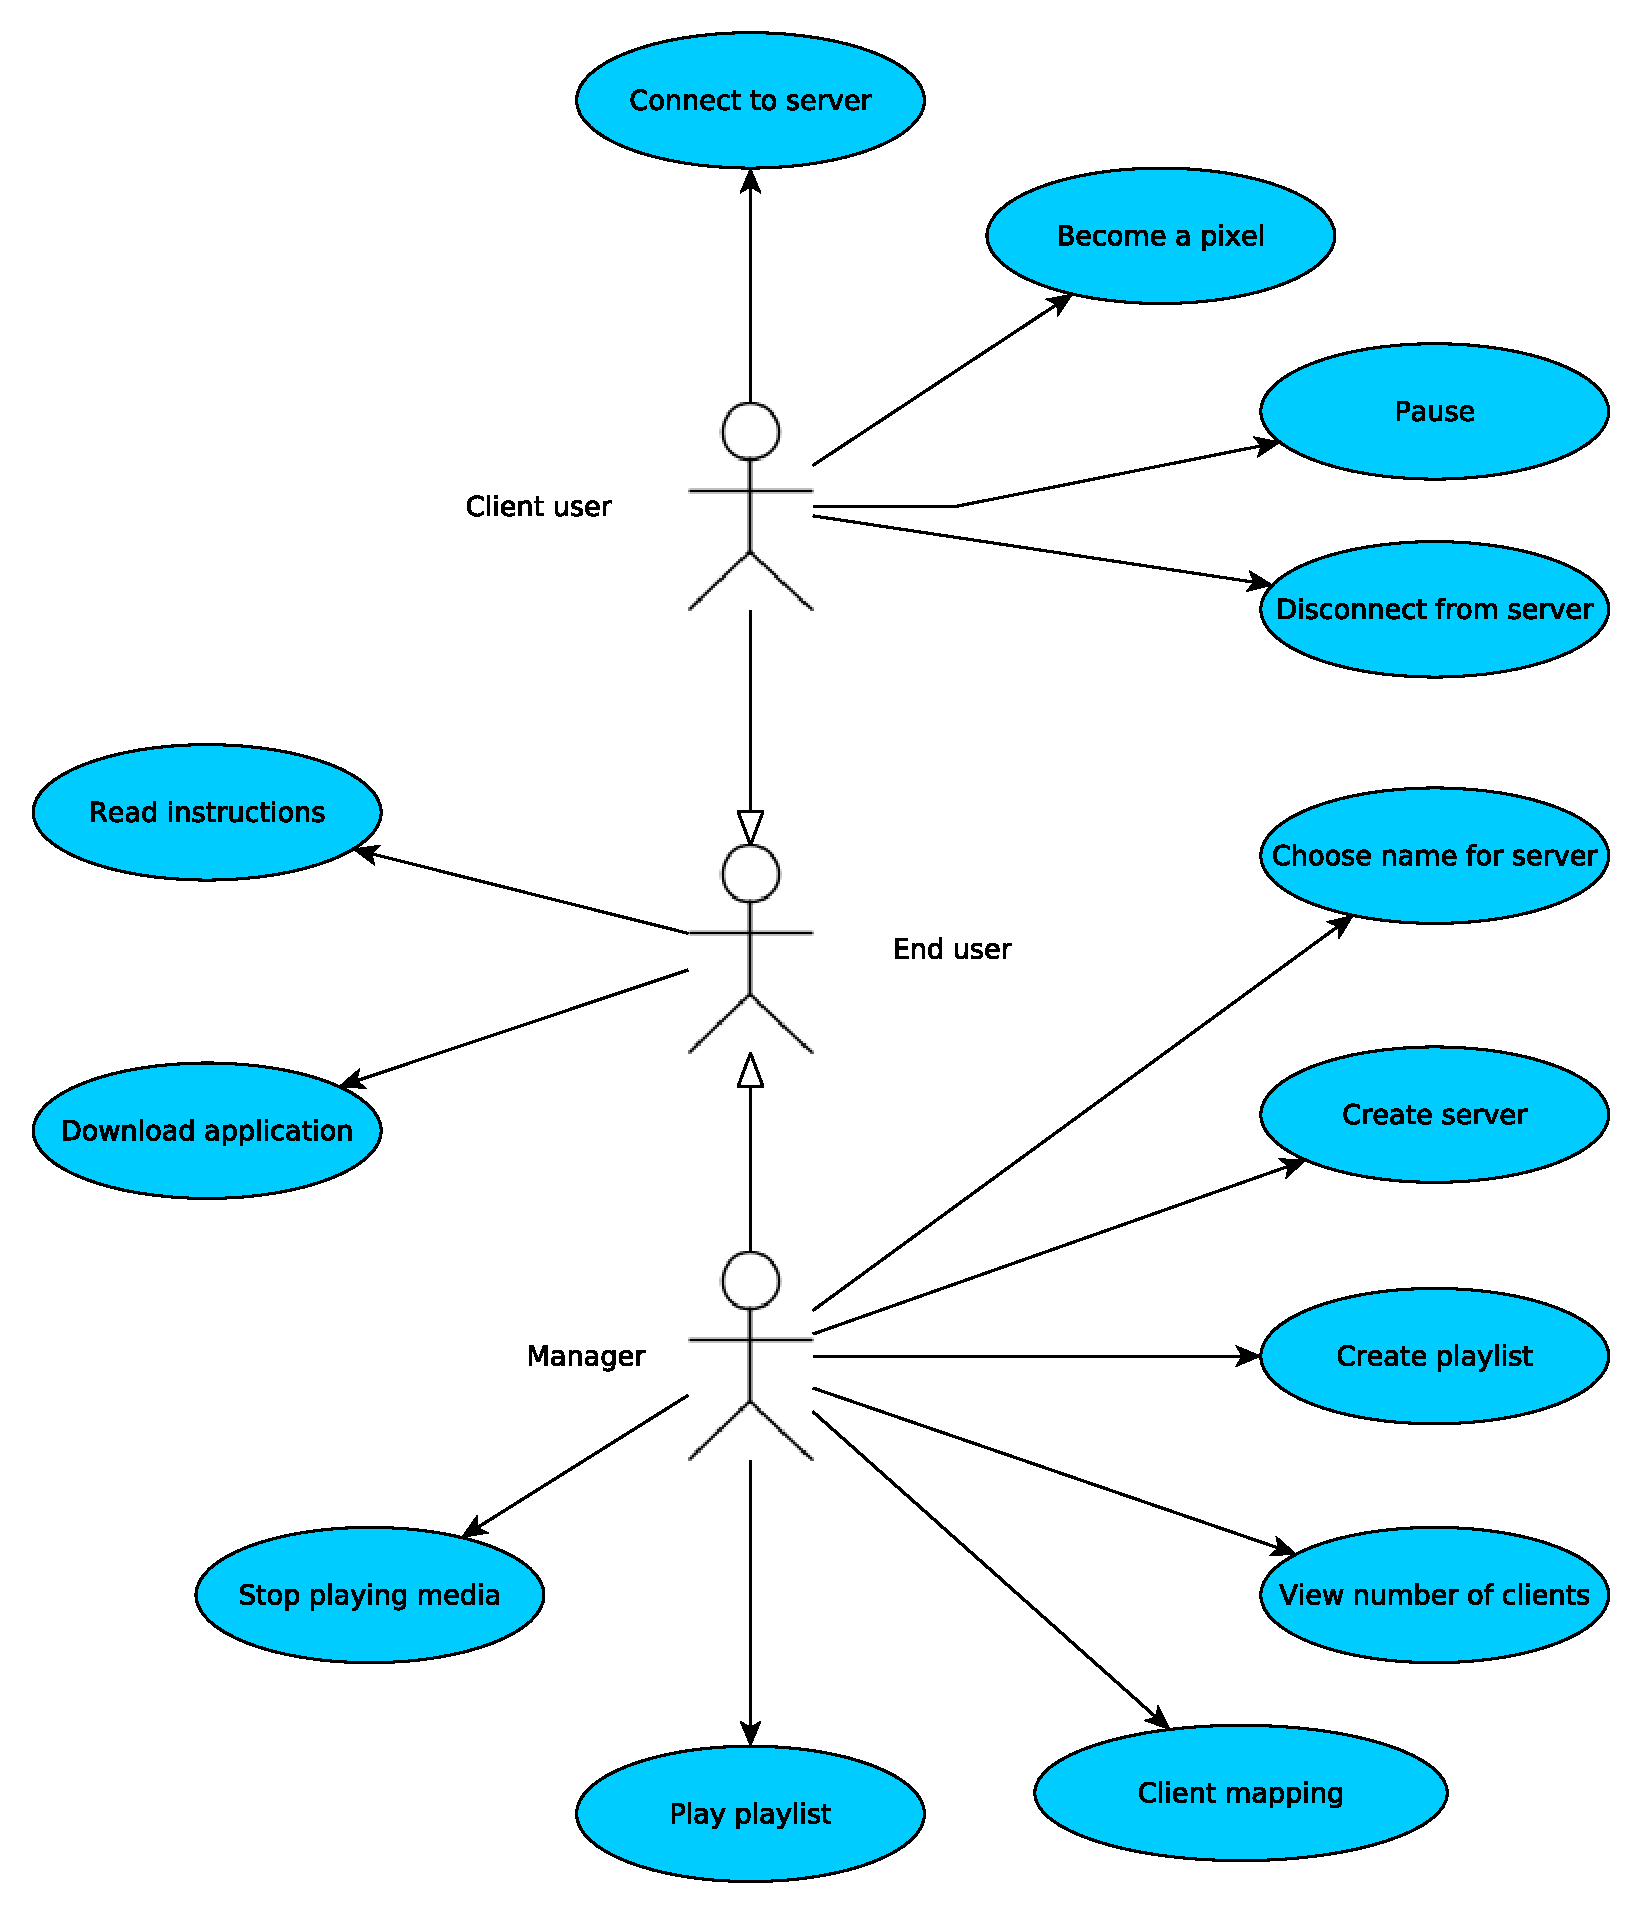
\includegraphics[scale=0.4]{images/usecase.pdf}
    \caption{Use case diagram depicting all actors.}
    \label{img:usecase}
    \end{center}
\end{figure}

You can see list of those requirements from end user's point of view below.

\begin{enumerate}
	\item[\textbf{E1}] \label{req_E1}
		I as a end user want to be able to read instructions.
	\item[\textbf{E2}] \label{req_E2}
		I as a end user want to be able to download relevant application from mobile application store.
\end{enumerate}

You can see list of functional requirements from client user's point of view below.
\begin{enumerate}
	\item[\textbf{C1}] \label{req_C1}
		I as a client user I want to easily choose to which server/concert stage I would like to connect.
	\item[\textbf{C2}] \label{req_C2}
		I as a client user I want to connect to chosen server.
	\item[\textbf{C3}] \label{req_C3}
		I as a client user I want to become a \emph{Pixel}.
	\item[\textbf{C4}] \label{req_C4}
		I as a client user I want to be able to pause being a Pixel.
	\item[\textbf{C5}] \label{req_C5}
		I as a client user I want to be able to disconnect from server/stage.
\end{enumerate}


You can see list of functional requirements from manager's point of view below.
\begin{enumerate}
	\item[\textbf{M1}] \label{req_M1}
		I as a manager I want to be able to choose name for my server/stage.
	\item[\textbf{M2}] \label{req_M2}
		I as a manager I want to be able to create a server.
	\item[\textbf{M3}] \label{req_M3}
		I as a manager I want to be able view attendance.
	\item[\textbf{M4}] \label{req_M4}
		I as a manager I want to be able to start mobile phone localization.
	\item[\textbf{M5}] \label{req_M5}
		I as a manager I want to be able to choose playlist to be played.
	\item[\textbf{M6}] \label{req_M6}
		I as a manager I want to be able to start playing given media.
	\item[\textbf{M7}] \label{req_M7}
		I as a manager I want to be able to start pause playing the media.
	\item[\textbf{M8}] \label{req_M8}
		I as a manager I want to be able to start pause stop the media.
\end{enumerate}

\subsection{Non-functional}
You can see non-functional requirements listed below.

\begin{enumerate}
\item[\textbf{N1}] \label{req_N1} Product must work as a server and client architecture.
\item[\textbf{N2}] \label{req_N2} Client side application must work on Android platform.
\item[\textbf{N3}] \label{req_N3} Application must be deployed to Google Play application store.
\item[\textbf{N4}] \label{req_N4} The product must be scalable -- it must work with  different count of mobile phones and it must support at least 16 client devices.
\end{enumerate}

\subsubsection{Quality attributes}
\phantomsection
\label{sec:quality_attributes}

\paragraph{Accessibility}
is the degree to which a the product is available to as many people as possible. 
Accessibility can be viewed as the "ability to access" and benefit from the product. 
To achieve this we plan to release the product on the Android Play Store, and we are also using TestFlight to make the applications as accessible as we can.

\paragraph{Interoperability}
describes the extent to which systems and devices can exchange data, and interpret that shared data. Digital Lighter server and client application should be able to mutually share specific structure or format of data that is preserved and unalterd during the process.  

\paragraph{Maintainability}
is the ease with which a product can be maintained. This means the product needs to isolate defects or their cause, prevent unexpected breakdowns, correct defects and repair or replace faulty components. If one component need to be replaced, then the system should do this without having to replace still-working parts. The product also needs make future maintenance easy.

\paragraph{Modifiability}
is all about handling changes, and this is including the extent to which this modification affects other functions. 
Code must be prepared for changes, and this can only be done by increase cohesion, and reduce coupling. 
If the modules get built smaller, the risk of having to make a change will be reduced. 
Team should also make sure that dependencies are restricted. 
Increasing the cohesion, or interdependency within modules, can affect build time, load time, initialization time or run time, therefore some trade-offs have to be done.

\paragraph{Performance}
is about managing system resources in the face of particular types of demands to achieve acceptable timing behavior. 
Performance can be measured in terms of throughput and latency. 
Performance can be improved by reducing demand, or by managing resources more appropriately. 
Reducing demands will have the side effect of reducing fidelity, or refuse service to some requests. 
Managing the resources more fitting can be done through scheduling, relication, or simply increase the resources available.

WRITE MORE HERE WEHN WE KNOW MORE!!


\paragraph{Usability}
Usability is the ease of use and learnability of the product.
Usability includes methods of measuring usability, such as analysis of needs or the study of the principles behind an object's perceived efficiency or elegance. We want our product to be easy to use, understandable, and easy to learn.  

\section{Summary}
In this chapter it was explained how the application's basic life-cycle looks like and the use case diagram \ref{img:usecase} was introduced.
According to use case diagram \ref{img:usecase} there were created \emph{Epics} which serve as a requirements. 
After that non-functional requirements were introduced.
In following chapters each user story which is connected to relevant requirement will be referenced with requirement's identification.

As you could see, client user's interaction with both applications is rather simple (and as the customer suggested the user interface is not core of the work) the main attention will be focused on image processing, network programming, synchronization and mapping devices into screen.

\begin{figure}[!ht]
    \begin{center}
    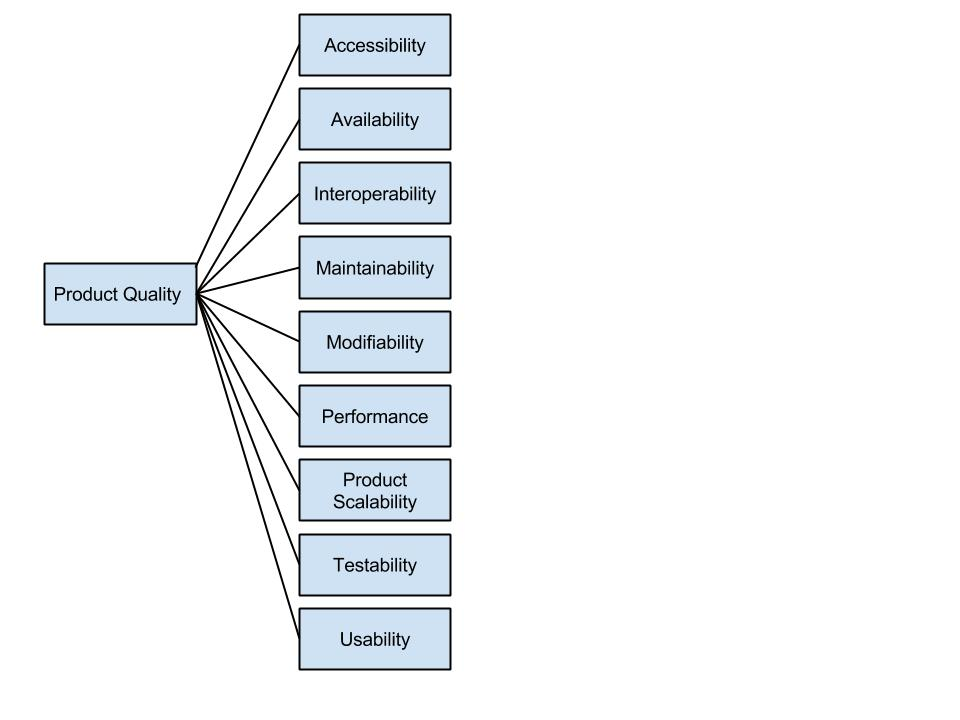
\includegraphics[scale=0.4]{images/qualityAttributes.jpg}
    \caption{Quality attributes.}
    \label{img:qualityAttributes}
    \end{center}
\end{figure}